%%%%%%%%%%%%%%%%%%%%%%%%%%%%%%%%%%%%%%%%%%%%%%%%%%%%%%%%%%%%%%%%%%%%%%%%%%%%%
%%% Programme for the EuBIC winter School 2017
%%%%%%%%%%%%%%%%%%%%%%%%%%%%%%%%%%%%%%%%%%%%%%%%%%%%%%%%%%%%%%%%%%%%%%%%%%%%%

\pdfminorversion=4
\documentclass[a5paper,10pt,oneside]{article}
\usepackage[a5paper, top=1cm, bottom=2cm, left=1cm, right=1cm]{geometry}
\usepackage[T1]{fontenc}
\usepackage[utf8]{inputenc}
\usepackage{changepage}
\usepackage{emptypage}
\usepackage{listingsutf8}
\usepackage{graphicx}
\usepackage[dvipsnames,table]{xcolor}
\usepackage[small,bf,margin=1cm,singlelinecheck=true]{caption}
\usepackage{layout}
\usepackage{hyperref}
\usepackage[ddmmyyyy,hhmmss]{datetime}
\usepackage{tabularx}
\usepackage{multirow}

% set font family
\usepackage{lmodern}
\renewcommand*\rmdefault{lmss}

\title{EuBIC Winter School 2017}
\author{EuBIC Winter School Organizers}

\begin{document}

\definecolor{eubicRed}{HTML}{c00418}
\definecolor{eubicGray}{HTML}{777777}

\newcolumntype{L}[1]{>{\raggedright\let\newline\\\arraybackslash\hspace{0pt}}m{#1}}
\newcolumntype{C}[1]{>{\centering\let\newline\\\arraybackslash\hspace{0pt}}m{#1}}
\newcolumntype{R}[1]{>{\raggedleft\let\newline\\\arraybackslash\hspace{0pt}}m{#1}}

\newcommand{\mysection}[2]{
  \setcounter{section}{#1}
  \color{eubicRed}
  \section*{#2}
  \addcontentsline{toc}{section}{#2}
  \color{black}
}

\begin{center}
  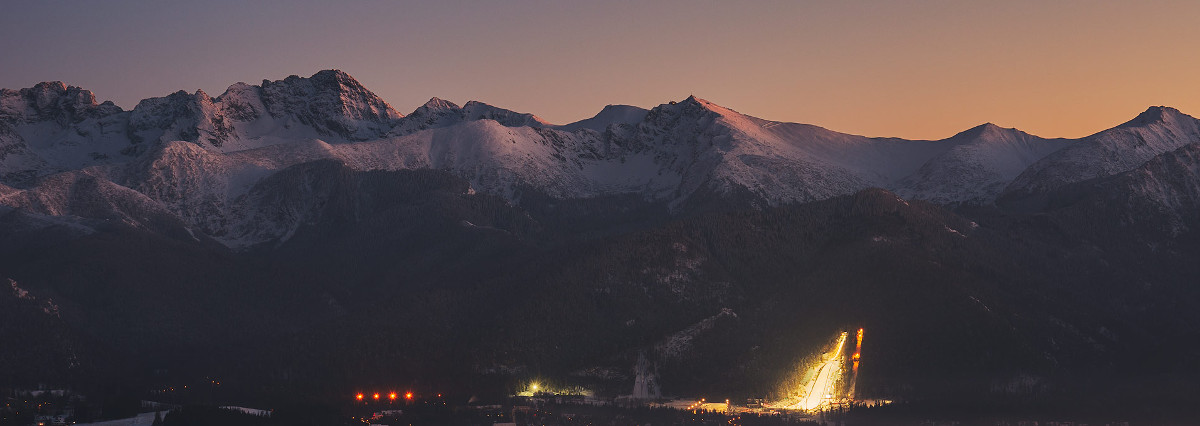
\includegraphics[width=\textwidth]{graphics/ski-jumping-wallpapers-small.jpg}\\
  \vspace*{\fill}
  {\huge \color{eubicRed} \textbf{EuBIC Winter School 2019}}\\[1.0cm]
  {\color{eubicGray} 15th -- 18th January 2019, Hotel Mercure Kasprowy, Zakopane, Poland}\\[1.0cm]
  \raisebox{-.3\height}{
\includegraphics[width=0.2\textwidth]{graphics/eubic_logo.png}}
  \hspace*{0.2cm}
  {\LARGE \textbf{Programme}}
  \hspace*{0.2cm}
  \raisebox{-.3\height}{
\includegraphics[width=0.2\textwidth]{graphics/eupa-logo.png}}\\[1.5cm]
  \href{https://www.proteomics-academy.org/eubic-winter-school-2019}{https://www.proteomics-academy.org/eubic-winter-school-2019}
\end{center}
\vspace*{\fill}

\pagebreak
\mysection{1}{Day 1 -- 15. January 2019}
\noindent\textbf{Educational Day}

\begin{table}[!h]
  \centering
  \begin{tabular}{ | L{0.1\textwidth} | C{0.26\textwidth} | C{0.26\textwidth} | C{0.26\textwidth} | }
    \hline
    \multicolumn{1}{|c|}{\textbf{Time}} & \multicolumn{3}{c|}{\textbf{Title}} \\
    \hline
    09:30 - 10:00 & \multicolumn{3}{c|}{Welcome coffee \& Registration} \\
    \hline
    10:00 - 10:30 & \multicolumn{3}{c|}{Opening Session} \\
    \hline
    10:30 - 12:00 & \cellcolor{LimeGreen} Introduction to computational mass spectrometry using OpenMS, Part I &
                    \cellcolor{Goldenrod} Computational introduction into DIA &
                    \cellcolor{Melon} Label-free quantification: concepts and algorithms \\
    \hline
    12:00 - 13:00 & \multicolumn{3}{c|}{\color{eubicGray}Lunch Break} \\
    \hline
    13:00 - 14:30 & \cellcolor{LimeGreen} Introduction to computational mass spectrometry using OpenMS, Part I (continued) &
                    \cellcolor{Goldenrod} Computational introduction into DIA (continued) &
                    \cellcolor{RedOrange} Quantitative proteomics: statistics, clustering and complexes \\
    \hline
    14:30 - 14:45 & \multicolumn{3}{c|}{\color{eubicGray} Coffee Break} \\
    \hline
    14:45 - 16:15 & \cellcolor{Aquamarine} Introduction to computational mass spectrometry using OpenMS, Part II &
                    \cellcolor{Goldenrod} Computational introduction into DIA (continued) &
                    \cellcolor{RedOrange} Quantitative proteomics: statistics, clustering and complexes (continued) \\
    \hline
    16:15 - 16:30 & \multicolumn{3}{c|}{\color{eubicGray} Coffee Break} \\
    \hline
    16:30 - 18:00 & \cellcolor{Aquamarine} Introduction to computational mass spectrometry using OpenMS, Part II (continued) &
                    \cellcolor{Goldenrod} Computational introduction into DIA (continued) &
                    \cellcolor{RedOrange} Discussion about best practices and common pitfalls \\
    \hline
  \end{tabular}
\end{table}

\noindent For further information on the workshops, please see the electronic version of the programme or the winter school's webpage.

\pagebreak
\mysection{2}{Day 2 -- 16. January 2019}
\noindent\textbf{DIA and Standards}

\begin{table}[!h]
  \centering
  \begin{tabular}{ | L{0.1\textwidth} | C{0.6\textwidth} | C{0.2\textwidth} | }
    \hline
    \multicolumn{1}{|c|}{\textbf{Time}} & \textbf{Title} & \multicolumn{1}{c|}{\textbf{Speaker(s)}} \\
    \hline
    08:35 - 08:40  & \multicolumn{2}{c|}{Morning Welcome and Announcements} \\
    \hline
    08:40 - 09:25  & XCorDIA: a new database search engine to detect geentic variants from DIA data & Brian Searle  \\
    \hline
    09:25 - 10:10  & Developing the tools for the personalized medicine revolution: Using mass spectrometry for longitudinal molecular profiling & Hannes Röst \\
    \hline
    10:10 - 10:30  & \multicolumn{2}{c|}{\color{eubicGray}Coffee Break}  \\
    \hline
    10:30 - 11:15  & Label-free Quantification of Complex Proteomes using Ion-Mobility-based DIA & Stefan Tenzer  \\
    \hline
    11:15 - 12:00  & Bioinformatics for Proteomics - any open questions? & Martin Eisenacher  \\
    \hline
    12:00 - 13:00  & \multicolumn{2}{c|}{\color{eubicGray} Lunch Break}  \\
    \hline
    13:00 - 13:50  & \multicolumn{2}{c|}{Poster flash talks}  \\
    \hline
    13:50 - 14:20  & Sponsor talk & SVA \\
    \hline
    14:20 - 18:20  & Workshop Session (Coffee break at 15:30-15:50)             & see workshop descriptions  \\
    \hline
    18:20 - open end  & \multicolumn{2}{c|}{Poster Session \& Come Together}  \\
    \hline
  \end{tabular}
\end{table}

\begin{table}[h!]
  \centering
  \caption*{\textbf{Parallel Workshops}}
  \begin{tabular}{ L{0.23\textwidth} L{0.70\textwidth} }
    \rowcolor{LimeGreen}  \textbf{Stefan Tenzer}     & Quality Control and Benchmarking of Label-Free Quantification Workflows with LFQBench \\
    \rowcolor{Goldenrod}  \textbf{Martin Eisenacher} & The essentials before and after spectrum identification: Selecting the appropriate  database and inference strategy \\
    \rowcolor{Melon}      \textbf{ProFI}             & Discovering the open-source Proline software suite, a new efficient and user friendly solution for label-free quantification \\
    \rowcolor{Aquamarine} \textbf{Thermo}            & Proteome Discoverer 2.3 Workshop
  \end{tabular}
\end{table}


\pagebreak
\mysection{3}{Day 3 -- 17. January 2019}
\noindent\large\textbf{Result Interpretation}

\begin{table}[!h]
  \centering
  \begin{tabular}{ | L{0.1\textwidth} | C{0.6\textwidth} | C{0.2\textwidth} | }
    \hline
    \multicolumn{1}{|c|}{\textbf{Time}} & \textbf{Title} & \multicolumn{1}{c|}{\textbf{Speaker(s)}} \\
    \hline
    08:35 - 08:40  & \multicolumn{2}{c|}{Morning Welcome and Announcements} \\
    \hline
    08:40 - 09:25  & STRING -- Large-scale integration of data and text & Lars Juhl Jensen \\
    \hline
    09:25 - 10:10  & Prosit: Proteome-wide prediction of peptide tandem mass spectra by deep learning & Mathias Wilhelm \\
    \hline
    10:10 - 10:30  & \multicolumn{2}{c|}{\color{eubicGray}Coffee Break} \\
    \hline
    10:30 - 11:15  & Using phosphoproteomics data to study context-specific signalling & Evangelia Petsalaki \\
    \hline
    11:15 - 12:00  & Insights into the multi-functioning proteome
 & Kathryn Lilley \\
    \hline
    12:00 - 13:00  & \multicolumn{2}{c|}{\color{eubicGray} Lunch Break}  \\
    \hline
    13:00 - 13:30  & Sponsor Talk: Novel DIA Data Analysis Workflow: Integration of De Novo Sequencing and Database Search & BSI \\
    \hline
    13:30 - 17:30  & Workshop Session (Coffee break at 15:30-15:50) & see workshop descriptions  \\
    \hline
    17:30 - 18:00  & EuBIC Meeting & All new members are welcome \\
    \hline
    19:00 - open end & \multicolumn{2}{c|}{Social Event}  \\
    \hline
  \end{tabular}
\end{table}

\begin{table}[h!]
  \caption*{\textbf{Parallel Workshops}}
  \begin{tabular}{ L{0.23\textwidth} L{0.70\textwidth} }
    \rowcolor{LimeGreen}  \textbf{Lars Juhl Jensen}    & Network visualization with Cytoscape and stringApp \\
    \rowcolor{Goldenrod}  \textbf{Evangelia Petsalaki} & SELPHI: using data-driven approaches for analysis of phosphoproteomics datasets \\
    \rowcolor{Melon}      \textbf{Florian Meier}       & Advanced data acquisition methods with MaxQuant.Live \\
    \rowcolor{Aquamarine} \textbf{Matthias Wilhelm}    & Validation of peptide identifications \\
  \end{tabular}
\end{table}


\pagebreak
\mysection{4}{Day 4 -- 18. January 2019}
\noindent\textbf{Innovative methods}

\begin{table}[!h]
  \centering
  \begin{tabular}{ | L{0.1\textwidth} | C{0.6\textwidth} | C{0.2\textwidth} | }
    \hline
    \multicolumn{1}{|c|}{\textbf{Time}} & \textbf{Title} & \multicolumn{1}{c|}{\textbf{Speaker(s)}} \\
    \hline
    09:00 - 09:05  & \multicolumn{2}{c|}{Morning Welcome and Announcements} \\
    \hline
    09:05 - 09:50  & Ionbot: a novel, fully data-driven search engine for open modification and mutation searches & Sven Degroeve  \\
    \hline
    09:50 - 10:20  & \multicolumn{2}{c|}{YPIC - Young Proteomics Investigators Club} \\
    \hline
    10:20 - 10:50  & \multicolumn{2}{c|}{\color{eubicGray} Coffee Break}  \\
    \hline
    10:50 - 11:35  & Trapped ion mobility spectrometry: a new dimension for mass spectrometry-based proteomics & Florian Meier \\
    \hline
    11:35 - 12:00  & \multicolumn{2}{c|}{Announcement: Best Flash Talk, Best Poster Award, Closing Remarks} \\
    \hline
    12:00 - 12:45  & \multicolumn{2}{c|}{\color{eubicGray} Lunch}  \\
    \hline
    13:00          & \multicolumn{2}{c|}{\color{eubicGray} Shuttle Buses leaving}  \\
    \hline
  \end{tabular}
\end{table}

\color{eubicRed}
{\noindent \Large \textbf{Organizers}}
\addcontentsline{toc}{section}{Organizers}
\color{black}

\begin{table}[!h]
  \centering
  \begin{tabular}{ | L{0.47\textwidth} | L{0.47\textwidth} | }
    \hline
    Dominik Kopczynski

    Leibniz-Institut für Analytische Wissenschaften – ISAS – e.V.

    dominik.kopczynski@isas.de &
    Julian Uszkoreit

    Ruhr University Bochum

    julian.uszkoreit@rub.de \\
    \hline
    Wout Bittremieux

    University of Antwerp

    wout.bittremieux@uantwerpen.be &
    David Bouyssié

    Institute of Pharmacology and Structural Biology (CNRS)

    bouyssie@ipbs.fr \\
    \hline
    Viktoria Dorfer

    University of Applied Sciences Upper Austria

    viktoria.dorfer@fh-hagenberg.at &
    Marie Locard-Paulet

    Institute of Pharmacology and Structural Biology (CNRS)

    marie.locard@ipbs.fr\\
    \hline
    Veit Schwämmle

    University of Southern Denmark

    veits@bmb.sdu.dk &
    Alessio Soggiu

    Universita Delgi Studi di Milano

    alessio.soggiu@unimi.it \\
    \hline
    Sander Willems

    Ghent University

    sander.willems@ugent.be &
    \\
    \hline
  \end{tabular}
\end{table}


\pagebreak
\mysection{5}{Sponsors}
\textbf{Main sponsors:}
\begin{center}
  
\includegraphics[height=1.5cm]{graphics/eupa-logo}\hspace*{2cm}
  
\includegraphics[height=1.5cm]{graphics/ELS_Logo_Orange_RGB}
\end{center}
\vspace*{.5cm}
\noindent\textbf{Platinum sponsors:}
\begin{center}
  
\includegraphics[height=2cm]{graphics/Bioinformatics_Solutions_Inc__svg}
\end{center}
\vspace*{.5cm}
\noindent\textbf{Gold sponsors:}
\begin{center}
  
\includegraphics[height=1.5cm]{graphics/logo_ProFi}\hspace*{0.5cm}
  
\includegraphics[height=1.5cm]{graphics/thermo-logo}\hspace*{0.5cm}
  
\includegraphics[height=1.5cm]{graphics/sva_logo}
\end{center}
\vspace*{.5cm}
\noindent\textbf{General sponsor:}
\begin{center}
  
\includegraphics[height=1.5cm]{graphics/Molecular-Omics_logo}
\end{center}
\vspace*{.5cm}
\noindent\textbf{Associations supporting with grants:}
\begin{center}
  
\includegraphics[height=1.5cm]{graphics/logo_sfeap}\hspace*{1cm}
  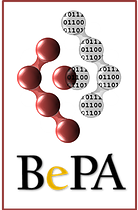
\includegraphics[height=1.5cm]{graphics/BePA_Logo}\hspace*{1cm}
  
\includegraphics[height=1.5cm]{graphics/apma_red-white_box_logo_1k}\hspace*{1cm}
  
\includegraphics[height=1.5cm]{graphics/LOGO_GANADOR_SEPROT_2016}
\end{center}

\end{document}
